\chapter{Cronograma}
\label{cap:cronograma}

Este capítulo registra a distribuição temporal das atividades desenvolvidas no TCC~1 e no TCC~2.

\section{Cronograma do TCC 1}

O TCC~1, desenvolvido de setembro a dezembro de 2025, concentrou-se na fundamentação teórica, na coleta e na análise exploratória dos dados do Distrito Federal. A Figura~\ref{fig:cronograma_tcc1} apresenta a distribuição das atividades, organizadas em quatro fases: planejamento da pesquisa, coleta e análise dos dados, metodologia e relatório.

\begin{figure}[htb]
	\centering
	\caption{Cronograma executado no TCC 1 (setembro a dezembro de 2025)}
	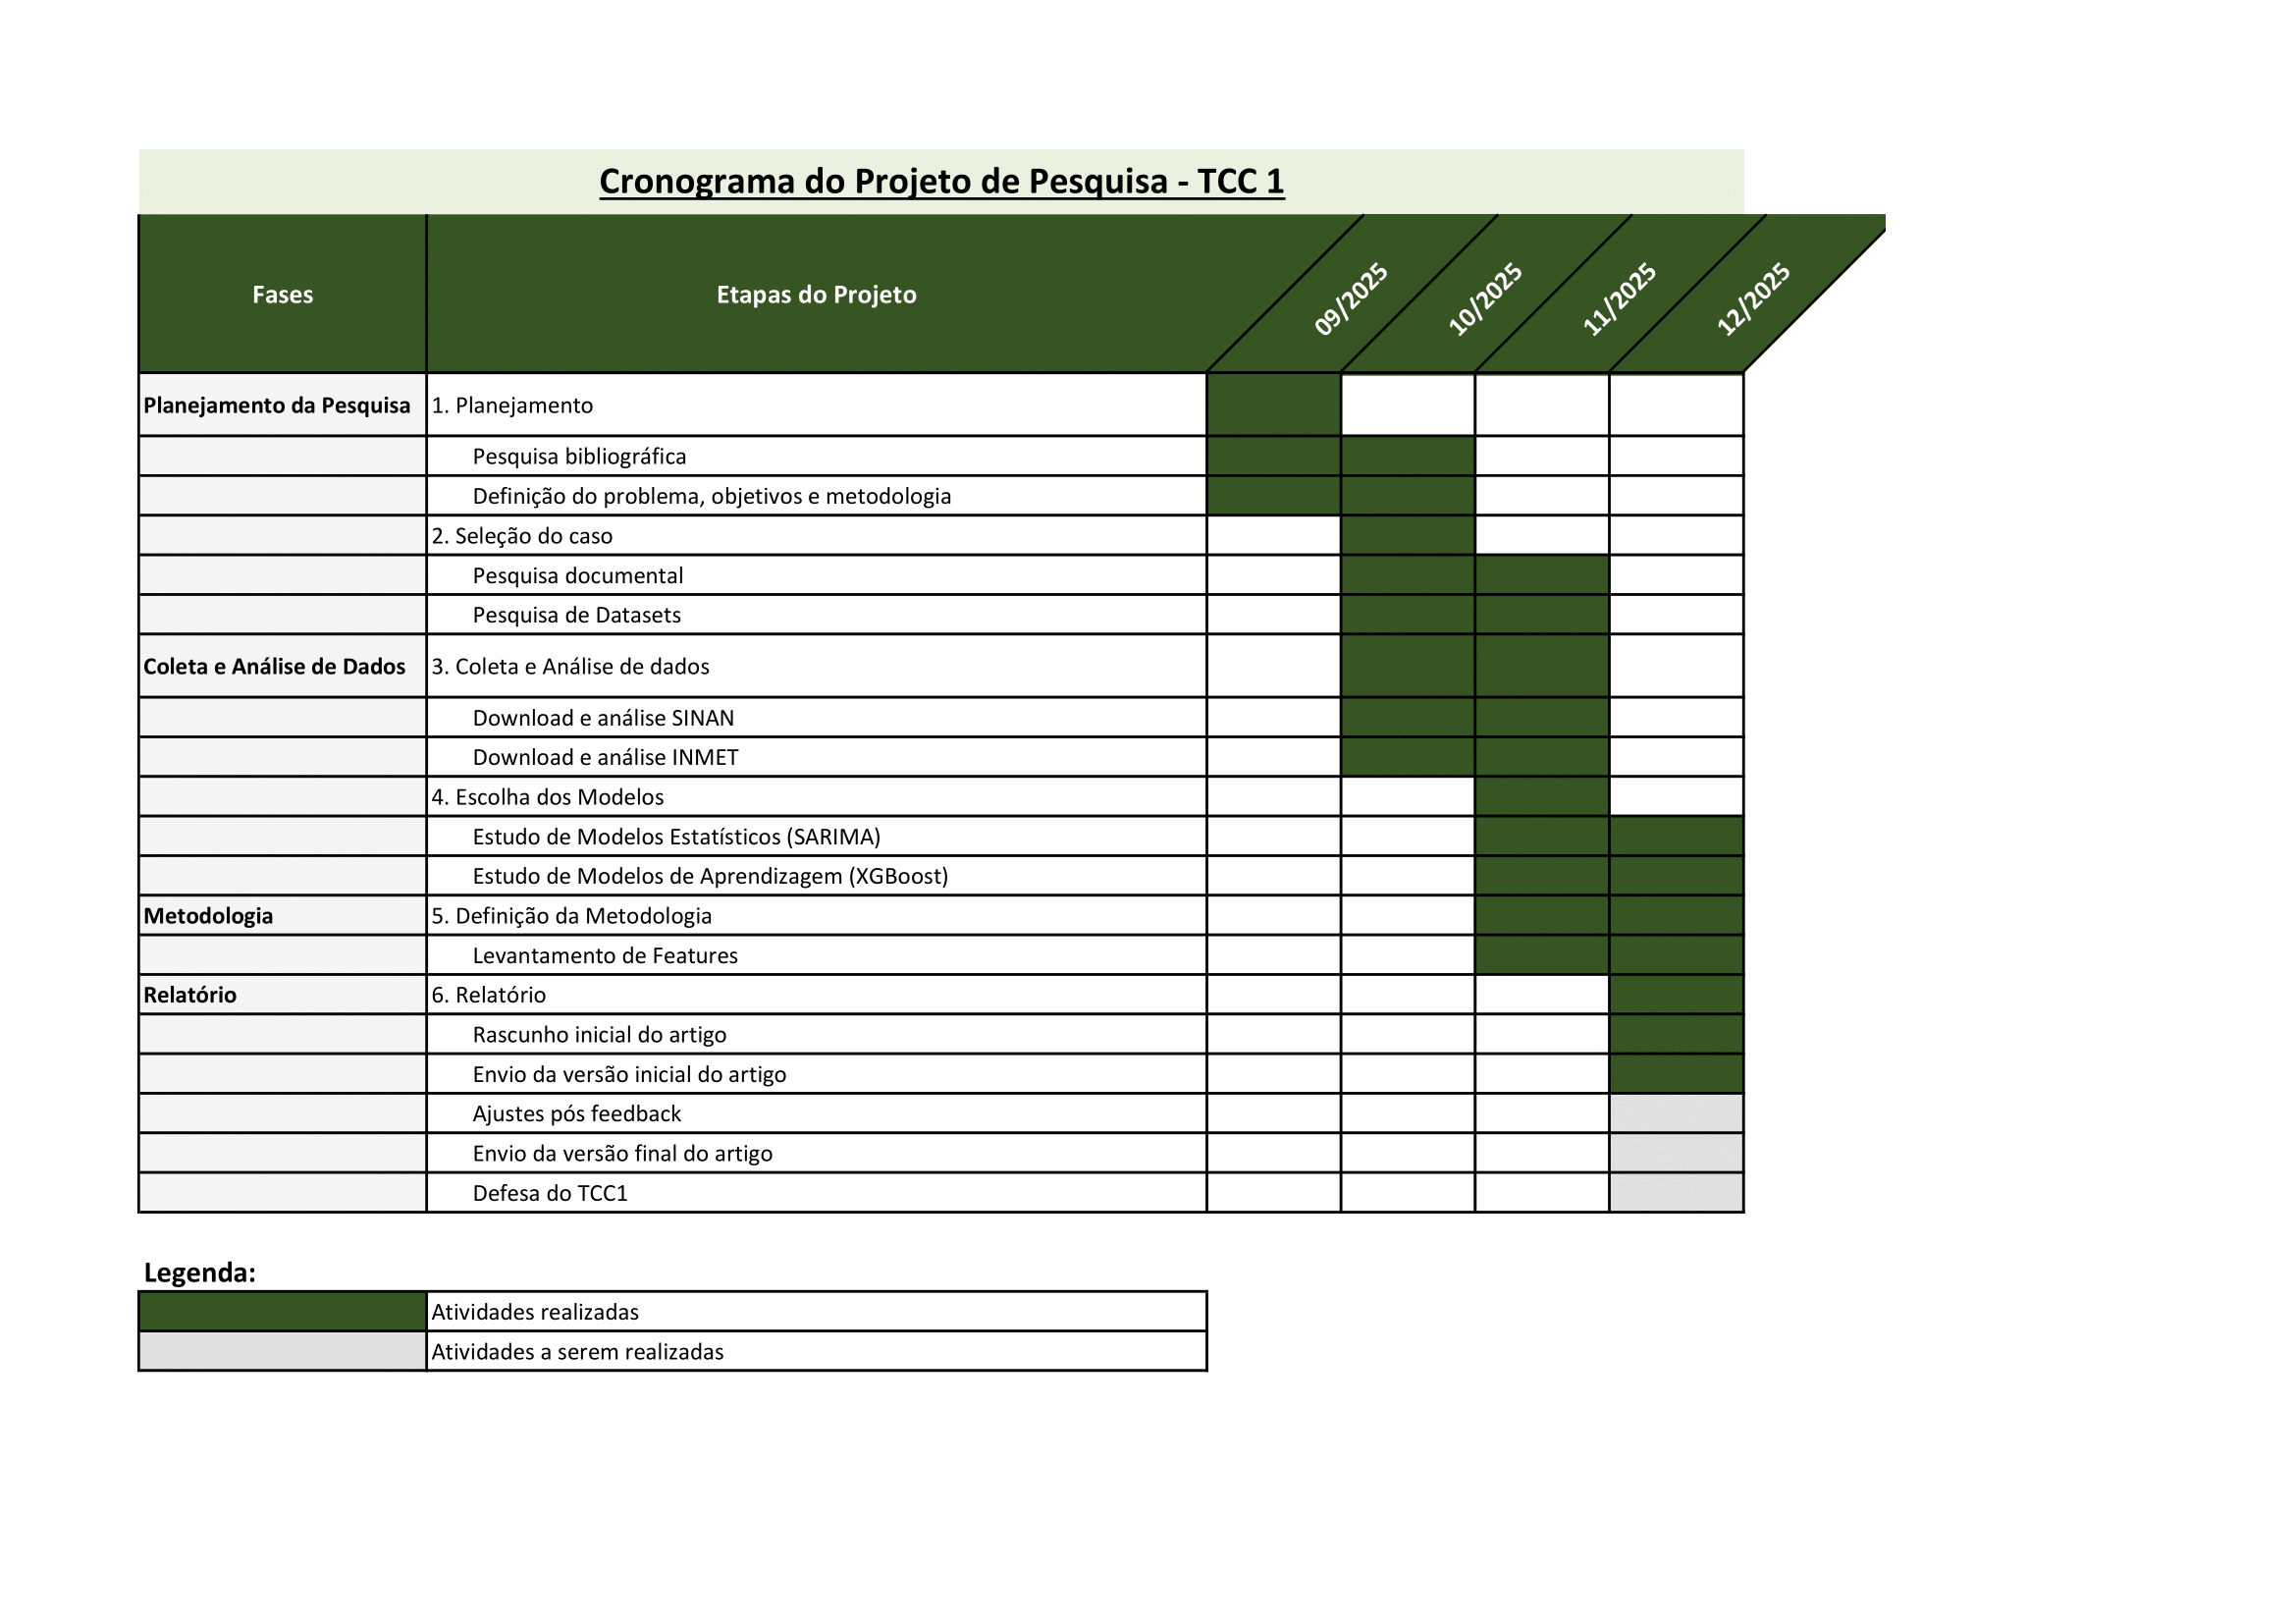
\includegraphics[width=\textwidth]{figuras/Cronograma_TCC1_2025-1.png}
	\label{fig:cronograma_tcc1}
	\fonte{Elaborado pelos autores.}
\end{figure}

\section{Cronograma Executado no TCC 2}

O TCC~2 havia sido planejado para o período de janeiro a março de 2026, com foco na comparação de diversas famílias de modelos para o Distrito Federal. A ampliação do escopo para o território nacional e a auditoria de qualidade dos dados estenderam a execução até setembro de 2026. A Tabela~\ref{tab:cronograma_tcc2} resume as atividades efetivamente realizadas, com as datas registradas no histórico de versões dos repositórios do projeto.

\begin{table}[htb]
\centering
\caption{Atividades executadas no TCC 2}
\label{tab:cronograma_tcc2}
\small
\begin{tabular}{|p{0.18\textwidth}|p{0.74\textwidth}|}
\hline
\textbf{Período} & \textbf{Atividades} \\ \hline
Mar. 2026 & Criação dos repositórios do TCC 2; notebooks de estudo de XGBoost e SARIMA \\ \hline
Abr. 2026 & Seleção de atributos climáticos por clusterização; integração do SINAN no recorte do Distrito Federal \\ \hline
Mai. 2026 & Pipeline nacional do SINAN (Bronze, Silver e Gold); pipeline do INMET e mapeamento estação--município; primeiros modelos XGBoost, SHAP e validação \textit{walk-forward} \\ \hline
Jun. 2026 & Reorganização dos repositórios; notebooks de treino no Colab e no Kaggle \\ \hline
Jul. 2026 & Modelo nacional em nível municipal, API REST e painel interativo \\ \hline
Set. 2026 & Pipeline com recorte de cinco anos; auditoria e correção dos dados do INMET e do SINAN; retreino com baselines; pipeline mesorregional; reprocessamento sobre os dados corrigidos; redação da monografia \\ \hline
\end{tabular}
\fonte{Elaborado pelos autores a partir do histórico dos repositórios.}
\end{table}

\section{Considerações sobre o Planejamento}

A principal diferença entre o planejado e o executado foi a ampliação do escopo, do Distrito Federal para todo o país, e a consequente substituição da comparação entre várias famílias de modelos por uma avaliação mais aprofundada de um único modelo frente a previsores ingênuos. A auditoria dos dados, não prevista no planejamento inicial, consumiu parte relevante do período final, mas foi determinante para a validade dos resultados.
